\documentclass[a4paper]{article}
%
\usepackage{graphicx,tikz}
\usepackage{amsmath,amssymb}
\usepackage[hidelinks]{hyperref}
\usepackage{xcolor}
\usepackage{framed}
%
\renewenvironment{leftbar}[1][\hsize]
{%
    \def\FrameCommand
    {%
        {\color{red}\vrule width 2pt}%
        \hspace{0pt}%must no space.
        \fboxsep=2pt\colorbox{yellow}%
    }%
    \MakeFramed{\hsize#1\advance\hsize-\width\FrameRestore}%
}
{\endMakeFramed}
%
\graphicspath{{./figures/}}
%
\title{%
	\bfseries%
	{\large Numerical Techniques Practicum 1}\\[3ex]
	{\Large Getting started with LINUX and FORTRAN:}\\[1ex]
	{\Large Solving the oscillation equation.}
}
%
\author{Daan Degrauwe}
%
\addtolength\textwidth{4cm}
\addtolength\evensidemargin{-2cm}
\addtolength\oddsidemargin{-2cm}
\addtolength\voffset{-3cm}
\addtolength\textheight{5cm}
\setlength\parindent{0pt}
\setlength\parskip{5pt}
\setlength\parsep{5pt}
%
\usepackage{etoolbox}
\makeatletter
\preto{\@verbatim}{\topsep=2pt \partopsep=2pt }
%
\begin{document}
%
NOTES:
* copy/paste doesn't work from laptop => open guidelines in firefox in Desktop
* copy/pasting single quotes doesn't work => use double quotes everywhere
* add safety in run.sh for when compilation fails
* change compilation command in run.sh when moving to several files



\maketitle
%
\par
Most NWP and climate models are Fortran codes working on Linux machines. For this reason, the exercises and projects for the Numerical Techniques course will be given in such an environment.
%
\par
Since not all students are familiar with Linux and/or Fortran, this first practicum is conceived as a step-by-step exercise, where both Linux basics and Fortran basics are dealt with.
%
\par
The goal is to write a Fortran program that calculates a numerical solution for the oscillation equation, as given by
%
\begin{equation*}
	\frac{d\psi}{dt}=i\kappa\psi
\end{equation*}
%
with initial condition $\psi_{t=0}=1$. The exact solution is given by $\psi(t)=\exp(i\kappa t)$.
%
\par
For this exercise, it is assumed that you work on the HPC (High-Performance Computer) infrastructure of UGENT. The first thing to do (preferably \underline{before} the first practical session) is therefore to ask for an HPC account on \texttt{https://www.ugent.be/hpc/en/access/faq/access}. Afterwards, you should be able to login via \texttt{https://login.hpc.ugent.be}. This should give you an interface like
%
\begin{center}
	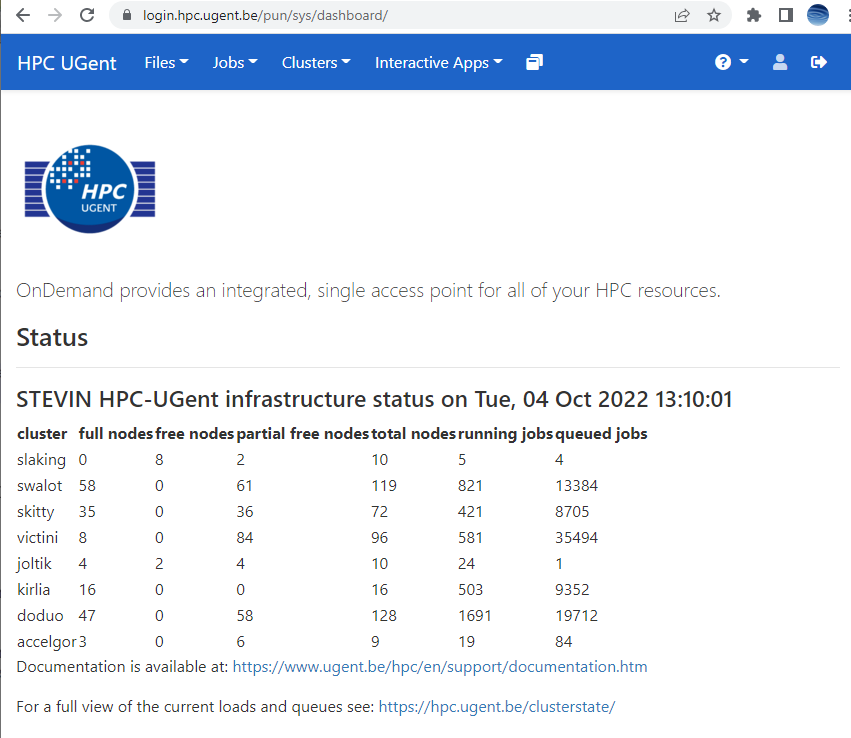
\includegraphics[scale=.4]{login_hpc}
\end{center}
%
\par
Different tools from this web platform will be used: the ``Files'' application to access files on the HPC, the ``Cluster Desktop'' application to enter a Linux desktop, and the ``Jupyter Notebook'' application for visualization of results.
%
\par
What is a bit peculiar about using HPC infrastructure is that nearly everything you do is done inside a `job'. This means that you first have to submit/launch your job, and once it starts you can begin your work.
%
\section{Accessing files}
%
\par
Under the ``Files'' application, hitting ``Home Directory'' should give you a graphical interface to your personal space on the HPC infrastructure. It lists all existing files and allows to download them, to upload new files, to view and edit (text) files, etc. However, in this practicum we'll work inside a Linux desktop to create/view/edit files. The Files application is mainly useful to exchange files with your local machine.
%
\section{Linux desktop}
%
\par
Launching a desktop job is done under ``Interactive Apps''-``Cluster Desktop''. Choose an appropriate time for your job (typically a few hours), and set the clustername to ``slaking''. Then hit the ``Launch'' button at the bottom. After a few minutes, you should see something like the following under ``My Interactive Sessions'':
%
\begin{center}
	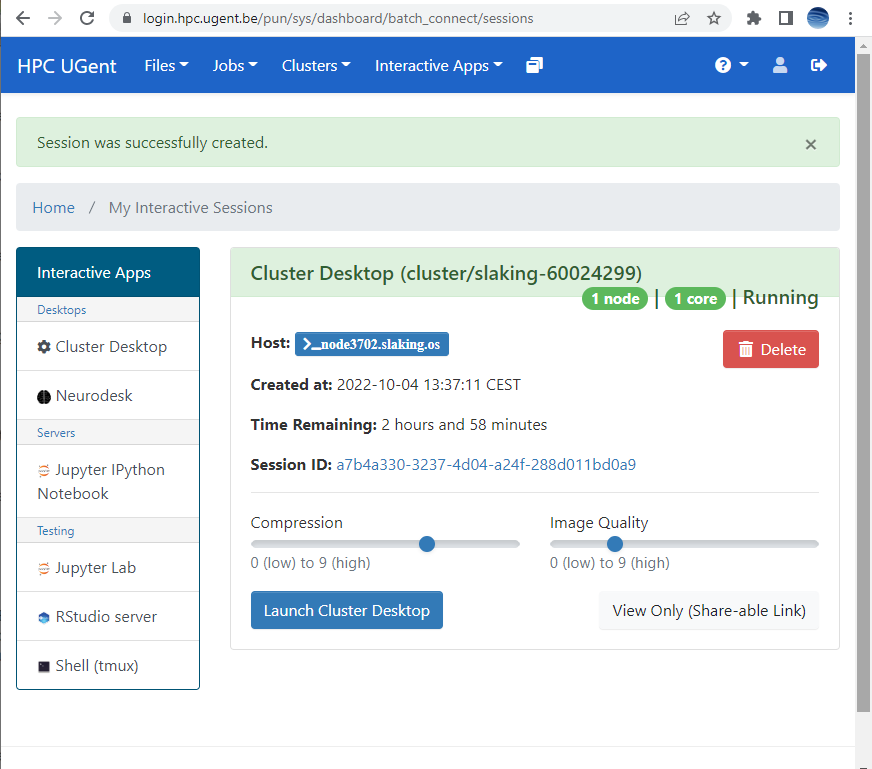
\includegraphics[scale=.4]{launch_desktop}
\end{center}
%
This means the job has started, and you can begin to work in it. Hit the ``Launch Cluster Desktop'' button to enter the desktop environment, which should look as follows:
%
\begin{center}
	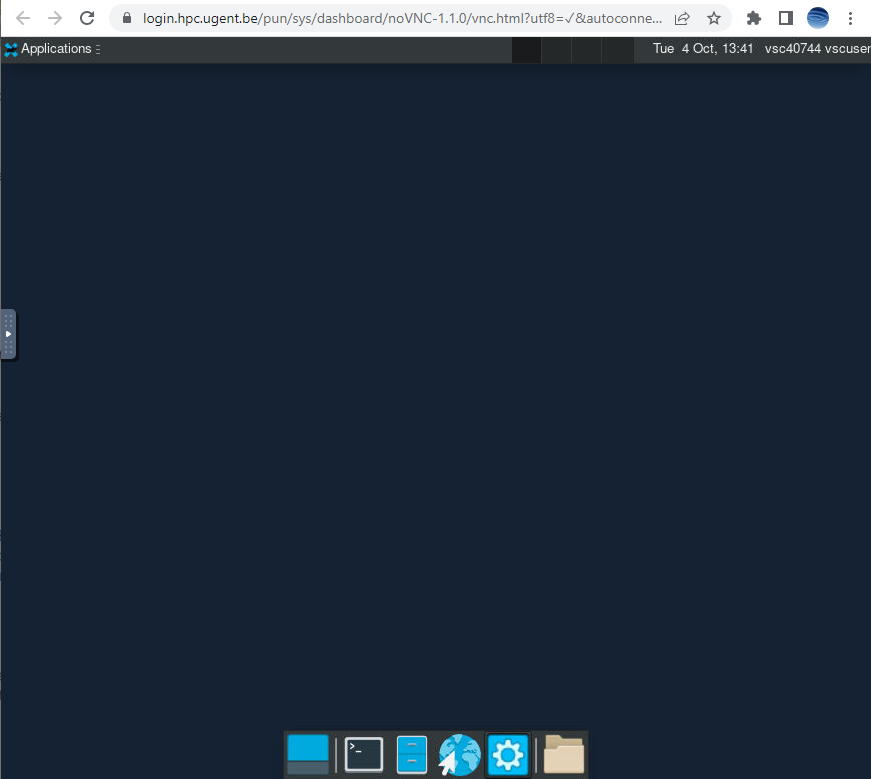
\includegraphics[scale=.4]{desktop}
	\begin{tikzpicture}
		\useasboundingbox (0,0);
		\draw [red, line width=2pt] (-5.5,.25) circle [radius=0.4];
		\draw [blue, line width=2pt] (-5,.25) circle [radius=0.4];
	\end{tikzpicture}
\end{center}
%
The most important applications in this desktop environment are the Linux terminal (red circle) and the File browser (blue circle).
%
\subsection{The file browser}
%
\par
This is just a convenient tool like Windows Explorer to browse and open files.
%
\subsection{The Linux terminal}
%
\par
Opening a Linux terminal gives you access to what is called the \emph{command line}. In Linux, almost everything you do is done by typing commands on the command line. For instance, try to execute the following command:
%
\begin{verbatim}
   $   date
\end{verbatim}
%
where the \texttt{\$} denotes that the command should be typed in the command line. The \texttt{\$} should not be typed itself! Hitting \texttt{ENTER} after this command prints the current date on the screen.
%
\par
Note: Linux is case-sensitive. This means that typing \verb+DATE+ or \verb+Date+ will not work.
%
\par
The Linux commands that are needed for this lesson will be explained during the course of the exercise. Appendix~\ref{sec:linux_commands} gives an overview of some of the most common Linux commands. At this point, you get following tricks for free:
%
\begin{itemize}
	\item Linux stores a history of commands you entered. To repeat a previous command, hit the \texttt{UP} arrow.
	\item Hitting the \texttt{TAB} key autocompletes. For example, if you type \texttt{dat}, and then hit \texttt{TAB}, it will autocomplete to \texttt{date}. This also works for files and directories. If multiple options exist for autocompletion, you can hit \texttt{TAB} twice, to see the options. For instance, if you type \texttt{cat}, and then hit \texttt{TAB} twice, you should see that \texttt{cat}, \texttt{catman} and \texttt{catchsegv} are possible commands.
\end{itemize}
%
\par
When working on a Linux command line, it is important to note that one works in a specific directory. Normally, this directory is visible before the \texttt{\$} symbol. $\sim$ denotes the home directory. You can also use the \verb+pwd+ command to print the working directory.
%
\subsection{Creating and modifying a text file}
%
\par
Creating and modifying text files is very important for the rest of this exercise (and the remainder of the course).
%
\par
On the command line, execute the following commands:
%
\begin{verbatim}
   $   mkdir ${HOME}/numtech
   $   cd ${HOME}/numtech
   $   touch test.txt
\end{verbatim}
%
Some explanation:
%
\begin{itemize}
	\item \texttt{mkdir} creates a new directory
	\item with \texttt{cd}, you go to this directory
	\item \texttt{touch} creates a (empty) file
\end{itemize}
%
To check if the file was indeed created, you can open the file browser and navigate to the newly created numtech directory, where the test.txt file should be visible. You can also check the contents of a directory from the command line with
%
\begin{verbatim}
   $   ls
\end{verbatim}
%
To modify a (text) file, select it in the file browser and double-click or hit Enter. This should launch a text editor (Geany) where you can modify the file as desired. Make sure to save a file after making modifications!
%
\par
Next, you can check the contents of a file with the following command in the command line:
%
\begin{verbatim}
   $   cat test.txt
\end{verbatim}
%
which should show you the text you entered in Geany. Finally, remove the test file with 
%
\begin{verbatim}
   $   rm test.txt
\end{verbatim}
%
\section{My first Fortran program}
%
\subsection{The Fortran code}
%
\par
First, create a directory for this program, and create an empty file \texttt{osceq.F90}:
%
\begin{verbatim}
   $   mkdir ${HOME}/numtech/osceq
   $   cd ${HOME}/numtech/osceq/
   $   touch osceq.F90
\end{verbatim}
%
\par
Open this file in Geany, and put the following Fortran code inside:
%
{\vspace{10pt}\hrule\small\vspace*{-2pt}\begin{verbatim}
	  PROGRAM OSCEQ
	  ! a program to solve the oscillation equation
	  
	  WRITE (*,*) "Welcome to the Oscillation Equation Solver."
	  
	  END PROGRAM OSCEQ
\end{verbatim}\hrule\vspace{5pt}}
%
Some explanations:
%
\begin{itemize}
	\item \verb+PROGRAM+ and \verb+END PROGRAM+ statements indicate the start and end of our program
	\item Text after a \verb+!+ denotes a comment. Use comments abundantly to make notes on the code.
	\item The \verb+WRITE+ statement is used to print text on the screen, or to write text to a file (see later). The argument \verb+(*,*)+ means that writing should be done to screen, in default formatting.
	\item Fortran is not case sensitive. This means it doesn't matter whether you write \verb+PROGRAM+ or \verb+program+ or \verb+PrOgRaM+.
\end{itemize}
%
\subsection{Compiling\label{sec:compile}}
%
\par
Before being able to execute Fortran code, it must be \emph{compiled}. This is the process of transforming a code that's readable to humans (Fortran) into a code that's readable to computers (executable files). For this, we use a \emph{compiler}.
%
\par
Compilation is quite easy (as long as your code doesn't contain any mistakes). We will use the \texttt{gfortran} compiler. To convert the Fortran code into an executable program, type the following in the command line:
%
\begin{verbatim}
	  $   gfortran osceq.F90 -o osceq
\end{verbatim}
%
This command tells \verb+gfortran+ the following: take the file \verb+osceq.F90+, convert it to an executable program, and put the result in the file \verb+osceq+.
%
\par
If all goes well, you should now have two files in the directory: \verb+osceq.F90+ and \verb+osceq+. You can check this with the Linux \verb+ls+ command. If you don't see the file \verb+osceq+, the compilation failed, most probably due to a coding mistake in the Fortran file. If you encounter errors during the compilation, try to understand what went wrong. Always look at the first error (later errors may be consequence of the first error). Ask for help if necessary: don't lose too much time on practicalities. You can use comments to indicate where you made a mistake in your program, in order to avoid such mistakes in the future.
%
\par
\textbf{Remark}: make sure to recompile the program after every modification of the Fortran file!
%
\subsection{Running\label{sec:run}}
%
\par
To execute the program, type the following on the command line:
%
\begin{verbatim}
   $   ./osceq
\end{verbatim}
%
This will print some text to screen.
%
\subsection{Automating tasks with Linux scripts}
%
\par
You may have noticed that recompiling and running often go together. It is therefore useful to create a Linux script that automates these two tasks. First create a file \texttt{run.sh}:
%
\begin{verbatim}
   $   touch run.sh
   $   chmod +x run.sh
\end{verbatim}
%
Where the \verb+chmod+ command marks the file as an executable script.
%
\par
Next, open this file in Geany, and put the following text in it:
%
{\vspace{10pt}\hrule\small\vspace*{-2pt}\begin{verbatim}
    # Script to compile and run the oscillation equation program
    
    # remove executable file
    rm osceq
    
    # Compile
    echo "Compiling"
    gfortran -o osceq osceq.F90
    
    # Run
    echo "Running"
    ./osceq
\end{verbatim}\hrule\vspace{5pt}}
%
%
Some explanations:
%
\begin{itemize}
	\item Comments in Linux scripts are indicated by a \verb+#+.
	\item The \verb+rm+ command removes the existing executable.
	\item The \verb+echo+ command prints text to the screen.
\end{itemize}
%
\par
Running the script is done with
%
\begin{verbatim}
   $   ./run.sh
\end{verbatim}
%
\section{Defining and using variables in Fortran}
%
\par
Let us now introduce some variables in our Fortran program. However, before making further modifications, it is good practice to take a copy of the current directory:
%
\begin{verbatim}
   $   cd ..
   $   cp -r osceq/ osceq_v1
   $   cd osceq/
\end{verbatim}
%
With the first command, we move one directory up (so to \verb+${HOME}/numtech/+). The \verb+cp+ command takes a copy; to copy directories, the additional argument \verb+-r+ is required.
%
\par
Now we have stored a backup, we can proceed with modifying the source code. In Geany, change the file \texttt{osceq.F90} as follows:
%
{\vspace{10pt}\hrule\small\vspace*{-2pt}\begin{verbatim}
	  PROGRAM OSCEQ
	  ! a program to solve the oscillation equation
	  
	  IMPLICIT NONE       ! safety to make sure all variables are declared
	  
	  ! declarations
	  REAL    :: KAPPA    ! parameter kappa in the oscillation equation (frequency)
	  REAL    :: DT       ! timestep
	  INTEGER :: NT       ! number of timesteps
	  COMPLEX :: PSI0     ! initial condition

	  WRITE (*,*) "Welcome to the Oscillation Equation Solver."
	  
	  ! initialize parameters
	  KAPPA = 0.5
	  DT    = 1.0
	  NT    = 20
	  PSI0  = COMPLEX(1.0,0.0)      ! complex number 1.0 + 0.0 * i
	  
	  WRITE (*,*) 'Total integration time = ',NT*DT
	  WRITE (*,*) 'Courant number = ',KAPPA*DT
	  
	  END PROGRAM OSCEQ
\end{verbatim}\hrule\vspace{5pt}}
%
Compile and run this program by running the \verb+run.sh+ script.
%
\par
The program contains the following new ingredients:
%
\begin{itemize}
	\item The statement \verb+IMPLICIT NONE+ is a safety. It's good practice to put it in all your Fortran programs. It means that all variables should be declared explicitly.
	\item The statements \verb+REAL+, \verb+INTEGER+ and \verb+COMPLEX+ are used to \emph{declare} variables. Declaration is where you tell the compiler what kind a certain variable is. Besides REAL, INTEGER and COMPLEX, Fortran also knows CHARACTER and LOGICAL types.
	\item The variables are \emph{assigned} their values with the \verb+=+ operator.
	\item The variables can then be used in calculations as shown in the \verb+WRITE+ statements
\end{itemize}
%
\par
It is important to be aware of the types of variables. For instance, the numbers \verb+2+ and \verb+5+ are of type \verb+INTEGER+. This means that \verb+5/2+ will take value \verb+2+, because dividing two variables of type \verb+INTEGER+ results in another \verb+INTEGER+! To correctly perform divisions, make sure that one of the numbers is of type \verb+REAL+. For example, \verb+5.0/2+ will give you the desired \verb+2.5+.
%
\par
It should be mentioned that the organization of a Fortran program is quite strict: \emph{all} declarations should come before the executable statements. If you want to introduce a new variable, it should be declared at the beginning of the program, even if you only use it somewhere at the end.
%
\section{Loops}
%
\par
Now we get to the actual purpose of our program: the time integration. We will do this with the forward scheme, for which
%
\begin{equation*}
	\phi^{n+1}=(1+i\kappa\Delta t)\phi^n
\end{equation*}
%
\par
The time integration is a repetitive task: given the solution at the current timestep ($\phi^n$), the solution at the next timestep ($\phi^{n+1}$) is calculated. A repetitive task is implemented in Fortran with a \verb+DO+-loop.
%
\par
First, store a copy of your program with
%
\begin{verbatim}
   $   cd ..
   $   cp -r osceq/ osceq_v2
   $   cd osceq/
\end{verbatim}
%
\par
Then, modify the file \verb+osceq.F90+ as follows:
%
{\vspace{10pt}\hrule\small\vspace*{-2pt}\begin{verbatim}
	  PROGRAM OSCEQ
	  ! a program to solve the oscillation equation

	  IMPLICIT NONE       ! safety to make sure all variables are declared

	  ! declarations
	  REAL    :: KAPPA    ! parameter kappa in the oscillation equation (frequency)
	  REAL    :: DT       ! timestep
	  INTEGER :: NT       ! number of timesteps
	  INTEGER :: IT       ! current timestep
	  COMPLEX :: PSI0     ! initial condition
	  COMPLEX :: PSI, PHI ! exact and numerical time-solution
	  COMPLEX :: II       ! imaginary unit

	  ! initialize parameters
	  KAPPA = 0.5
	  DT    = 1.0
	  NT    = 20
	  PSI0  = COMPLEX(1.,0.)
	  II    = COMPLEX(0.,1.)

	  ! set initial conditions
	  IT=0
	  PSI=PSI0
	  PHI=PSI0
	  ! show values at zero'th timestep
	  WRITE (*,*) 't = ',IT*DT,'; PSI = ',REAL(PSI),'; PHI = ',REAL(PHI)

	  ! start loop over timesteps
	  DO IT = 1,NT

	    ! exact solution
	    PSI = EXP(II*KAPPA*DT)*PSI

	    ! numerical solution: forward scheme
	    PHI = (1+II*KAPPA*DT)*PHI

	    ! show values at current timestep
	    WRITE (*,*) 't = ',IT*DT,'; PSI = ',REAL(PSI),'; PHI = ',REAL(PHI)

	  ENDDO

	  END PROGRAM OSCEQ
\end{verbatim}\hrule\vspace{5pt}}
%
\par
New ingredients are:
%
\begin{itemize}
	\item The functions \verb+REAL()+ and \verb+EXP()+, which respectively take the real part of a complex number, and the exponential function
	\item The statements \verb+DO IT=1,NT+ and \verb+ENDDO+ denoting the start and end of a \emph{loop}. The enumerator \verb+IT+ takes the initial value of 1, and augments every timestep by 1, until it gets larger than \verb+NT+.
\end{itemize}
%
\par
When running the program, it should become clear that the forward scheme is unstable.
%
\section{Conditions}
%
\par
Conditional branching in Fortran is done with the \verb+IF+ statement. For instance, we could introduce the following piece of code to check for an unstable scheme:
%
{\vspace{10pt}\hrule\small\vspace*{-2pt}\begin{verbatim}
	  PROGRAM OSCEQ
	  ! a program to solve the oscillation equation
	  
	  ... (see previous version of the program)
	  
	  ! start loop over timesteps
	  DO IT = 1,NT
	  
	    ! numerical solution: forward scheme
	    PHI = (1+II*KAPPA*DT)*PHI
	    
	    ! warning if unstable
	    IF ( ABS(PHI) > 10.0 ) THEN
	      WRITE (*,*) 'WARNING: unstable behaviour detected'
	    ENDIF
	  
	  ENDDO
	  
	  END PROGRAM OSCEQ
\end{verbatim}\hrule\vspace{5pt}}
%
\par
When running long enough (\verb+NT+$\geq21$), you should see a warning in the output.
%
\par
More advanced conditions are achieved with \verb+.AND.+, \verb+.OR.+ and \verb+.NOT.+. If you want to execute some code when the condition is \emph{not} fulfilled, use the \verb+ELSE+ statement.
%
\section{Arrays}
%
\par
Arrays are collections of numbers. In this program, they allow to store the solution for the full time-range. Consider the following program:
%
{\vspace{10pt}\hrule\small\vspace*{-2pt}\begin{verbatim}
	  PROGRAM OSCEQ
	  ! a program to solve the oscillation equation

	  IMPLICIT NONE       ! safety to make sure all variables are declared

	  ! declarations
	  REAL    :: KAPPA    ! parameter kappa in the oscillation equation (frequency)
	  REAL    :: DT       ! timestep
	  INTEGER :: NT       ! number of timesteps
	  INTEGER :: IT       ! current timestep
	  COMPLEX :: PSI0     ! initial condition
	  COMPLEX :: II       ! imaginary unit
	  COMPLEX, ALLOCATABLE :: PSI(:), PHI(:) ! arrays of exact and numerical solution

	  ! initialize parameters
	  KAPPA = 0.5
	  DT    = 1.0
	  NT    = 100
	  PSI0  = COMPLEX(1.,0.)
	  II    = COMPLEX(0.,1.)

	  ! allocate memory for arrays
	  ALLOCATE(PSI(0:NT),PHI(0:NT))

	  ! set initial conditions
	  IT=0
	  PSI(IT)=PSI0
	  PHI(IT)=PSI0

	  ! start loop over timesteps
	  DO IT = 1,NT
	  	
	  	! exact solution
	  	PSI(IT) = EXP(II*KAPPA*DT)*PSI(IT-1)
	  	
	  	! numerical solution: forward scheme
	  	PHI(IT) = (1+II*KAPPA*DT)*PHI(IT-1)
	  	
	  ENDDO

	  ! show values
	  WRITE (*,*) 'PSI = ',REAL(PSI)
	  WRITE (*,*) 'PHI = ',REAL(PHI)

	  ! release memory
	  DEALLOCATE(PSI,PHI)

	  END PROGRAM OSCEQ
\end{verbatim}\hrule\vspace{5pt}}
%
\par
Working with arrays requires the following:
%
\begin{itemize}
	\item During the declaration, you should add the \verb+ALLOCATABLE+ attribute, and specify the number of dimensions. In this program, one-dimensional arrays are used, hence the \verb+(:)+. Two-dimensional arrays would be declared with \verb+(:,:)+
	\item The \verb+ALLOCATE+ statement tells the compiler what the size of the array should be, and makes sure the necessary memory is reserved for this array
	\item A single element of an array is accessed with the \verb+()+ construct. For instance, we calculate \verb+PHI(IT)+ from \verb+PHI(IT-1)+
	\item At the end, the reserved memory should be released with the \verb+DEALLOCATE+ statement.
\end{itemize}
%
\par
Quite important to remember when working with arrays is that you shouldn't exceed the limits of the array. For example, using \verb|PHI(NT+1)| in our program would lead to erroneous results or a crash of the program, because \verb+PHI+ was allocated with an upper bound of \verb+NT+. You can tell the compiler to detect such out-of-bound errors by compiling with the switch \verb+-fbounds-check+:
%
\begin{verbatim}
	  $   gfortran -fbounds-check osceq.F90 -o osceq
\end{verbatim}
%
\section{Subroutines and modules}
%
\par
For larger computer programs (NWP and climate models often contain millions of lines of code), it becomes necessary to organize the code in a structured way. This is achieved with \emph{subroutines}. A subroutine is a piece of code that can be called from somewhere else in the code.
%
\par
In principle, variables that are declared in the main part of the program are not known in the subroutine. Two mechanisms exist to transfer information to and from subroutines. Either by using \emph{arguments}, or by using \emph{global variables}. Global variables are implemented in Fortran by putting them in a \emph{module}.
%
\par
It is common practice to put all subroutines and modules in separate files.
%
\par
Let's organize our oscillation equation program in the following pieces:
%
\begin{itemize}
	\item a module \verb+CONSTANTS+ containing all constant variables;
	\item a subroutine \verb+SETUP_CONSTANTS+ to setup the values of these constant variables;
	\item a subroutine \verb+TIMELOOP+ to perform the time-loop;
	\item a subroutine \verb+WRITE_RESULT+ to write the results to a file;
	\item the main program, making calls to the other routines.
\end{itemize}
%
\par
Each of these pieces is put in a separate Fortran file. The file \verb+constants.F90+ contains
%
{\vspace{10pt}\hrule\small\vspace*{-2pt}\begin{verbatim}
	  MODULE CONSTANTS
	    ! a module contains global variables.
	    ! These are accessible from all subroutines and from the main program

	    IMPLICIT NONE

	    ! universal constants
	    COMPLEX :: II       ! imaginary unit

	    ! oscillation equation parameters
	    REAL    :: KAPPA    ! parameter kappa in the oscillation equation (frequency)
	    COMPLEX :: PSI0     ! initial condition

	    ! discretization variables
	    REAL    :: DT       ! timestep
	    INTEGER :: NT       ! number of timesteps

	  END MODULE CONSTANTS
\end{verbatim}\hrule\vspace{5pt}}
%
\par
The file \verb+setup_constants.F90+ contains
% 
{\vspace{10pt}\hrule\small\vspace*{-2pt}\begin{verbatim}
	  SUBROUTINE SETUP_CONSTANTS
	    ! subroutine to assign constants appropriate values

	    USE CONSTANTS       ! all variables from this module are now known in this subroutine

	    IMPLICIT NONE

	    II    = COMPLEX(0.,1.)

	    KAPPA = 0.5
	    PSI0  = COMPLEX(1.,0.)

	    DT    = 1.0
	    NT    = 100

	  END SUBROUTINE SETUP_CONSTANTS
\end{verbatim}\hrule\vspace{5pt}}
%
\par
The file \verb+timeloop.F90+ contains
% 
{\vspace{10pt}\hrule\small\vspace*{-2pt}\begin{verbatim}
	  SUBROUTINE TIMELOOP

	    USE CONSTANTS

	    IMPLICIT NONE

	    ! declare local variables
	    INTEGER              :: IT               ! current timestep
	    COMPLEX, ALLOCATABLE :: PSI(:), PHI(:)   ! arrays of exact and numerical solution

	    ! allocate memory for arrays
	    ALLOCATE(PSI(0:NT),PHI(0:NT))

	    ! set initial conditions
	    IT=0
	    PSI(IT)=PSI0
	    PHI(IT)=PSI0

	    ! start loop over timesteps
	    DO IT = 1,NT

	      ! exact solution
	      PSI(IT) = EXP(II*KAPPA*DT)*PSI(IT-1)

	      ! numerical solution: forward scheme
	      PHI(IT) = (1+II*KAPPA*DT)*PHI(IT-1)

	    ENDDO
	    
	    ! write the result
	    CALL WRITE_RESULT(PSI,PHI)
		
	    ! free memory
	    DEALLOCATE(PSI,PHI)

	  END SUBROUTINE TIMELOOP
\end{verbatim}\hrule\vspace{5pt}}
%
\par
The file \verb+write_result.F90+ contains
% 
{\vspace{10pt}\hrule\small\vspace*{-2pt}\begin{verbatim}
	  SUBROUTINE WRITE_RESULT(PSI,PHI)

	    ! write the result to a file
	    USE CONSTANTS

	    IMPLICIT NONE

	    ! arguments
	    COMPLEX, INTENT(IN) :: PSI(0:NT), PHI(0:NT)
	    
	    ! auxiliary results
	    INTEGER :: IT     ! timestep

	    ! open a file
	    OPEN(FILE='output.dat',UNIT=20)
	    
	    ! write heading
	    WRITE (20,'(A6,A16,A16)') 'time','exact','numerical'
	    
	    ! write solutions at all timesteps to the file
	    DO IT=0,NT
	      WRITE (20,'(F6.2,E16.8,E16.8)') IT*DT, REAL(PSI(IT)), REAL(PHI(IT))
	    ENDDO
	    
	    ! close the file
	    CLOSE(UNIT=20)

	  END SUBROUTINE WRITE_RESULT
\end{verbatim}\hrule\vspace{5pt}}
%
\par
And finally, the file \verb+osceq.F90+ contains
% 
{\vspace{10pt}\hrule\small\vspace*{-2pt}\begin{verbatim}
	  PROGRAM OSCEQ
	    ! a program to solve the oscillation equation

	    IMPLICIT NONE
	    
	    ! initialize constant parameters
	    CALL SETUP_CONSTANTS()

	    ! time loop
	    CALL TIMELOOP()

	  END PROGRAM OSCEQ
\end{verbatim}\hrule\vspace{5pt}}
%
\par
The compilation of multiple files is done as follows:
%
{\small\begin{verbatim}
	  $   gfortran constants.F90 setup_constants.F90 timeloop.F90 write_result.F90 osceq.F90 -o osceq
\end{verbatim}}
%
\par
Remarks and new concepts:
%
\begin{itemize}
	\item One can hardly say that our program became simpler by reorganizing into subroutines. However, each of the building blocks is quite simple in itself. It's much easier to find your way through the program now.
	\item Calling a subroutine is done with the \verb+CALL+ statement. 
	\item Arguments have an \verb+INTENT+ attribute, which specifies whether it's an input (\verb+IN+) or an output argument (\verb+OUT+).
	\item It's very important that the argument declaration in the subroutine matches the argument that is passed in the \verb+CALL+ statement! You will get strange behaviour if this is not the case. `Matching' means that the type (\verb+COMPLEX+, \ldots) should be the same, as well as the dimension if it's an array.
	\item To make global variables accessible in a subroutine, the \verb+USE+ statement should be used.
	\item Writing to a file is done in three steps:
		\begin{enumerate}
			\item open the file with the \verb+OPEN+ statement. The filename is specified, and a \emph{unit} number is assigned. You can freely choose this unit, as long as it is not in use for another file. You also shouldn't take 0, 1 or 6 as unit number.
			\item write stuff to the file with the \verb+WRITE+ statement. Specify the unit number of the file you want to write to, as well as the \emph{format}. The code shows how to specify the formats for character strings and for floating point real numbers.
			\item close the file with the \verb+CLOSE+ statement.
		\end{enumerate}
	\item for the compilation, it's important to put the Fortran files containing modules (in our case\\ \verb+constants.F90+) \emph{before} the Fortran files using these modules.
\end{itemize}
%
\section{Visualizing the output in a Jupyter Notebook}
%
\par
Fortran is a programming language that's intended to perform calculations. Visualizing results is commonly done with other programs, such as Matlab, R, gnuplot, python, etc. All of these programs are capable of reading numerical data from a file (like the one created by our program). For this course, we will use a Jupyter Notebook to postprocess (visualize and inspect) the results of our calculations.
%
\subsection{Launching a Jupyter Notebook}
%
\begin{enumerate}
	\item Head back to \texttt{https://login.hpc.ugent.be/}
	\item Under ``Interactive Apps'', select ``Jupyter IPython Notebook''
	\item Select slaking as the cluster, and select {\bfseries ``\texttt{7.15.0 foss 2020a Python 3.8.2}''} as the IPython version. Then hit the ``Launch'' button.
	\item After a few minutes, the Jupyter Notebook session should appear in your ``My Interactive Sessions'' panel. Then hit the ``Connect to Jupyter Notebook'' button, which should launch the Jupyter browser in a new tab.
	\item Browse to the \texttt{numtech/osceq} directory that you've been working in so far, and hit ``New''--``Python 3'' to create a new notebook.
	\item Rename the notebook from the default `Untitled' to something more appropriate, e.g. `osceq'.
\end{enumerate}
%
\subsection{Working in a Jupyter Notebook}
%
\par
A notebook is organized in `cells', which are pieces of python code that can be executed by hitting Shift+Enter. After modifying the content of a cell, make sure to rerun it.
%
\par
In the first cell, we'll load some necessary libraries:
%
\begin{verbatim}
    # load some libraries
    %matplotlib inline
    import numpy as np
    import matplotlib.pyplot as plt
\end{verbatim}
%
\par
In the following cell, we'll load the data from the \texttt{output.dat} file
%
\begin{verbatim}
    # read the output data
    filename='output.dat'
    data=np.loadtxt(filename,skiprows=1)
    # select columns
    t=data[:,0]
    y_exact=data[:,1]
    y_numerical=data[:,2]
\end{verbatim}
%
\par
Next, we can visualize the results in the next cell with
%
\begin{verbatim}
    # open a figure
    fig, ax = plt.subplots(figsize=(12,8))
    # plot exact and numerical result
    plt.plot(t,y_exact,label='exact')
    plt.plot(t,y_numerical,label='numerical')
    # add legend
    plt.legend();
\end{verbatim}
%
\section{Exercises}
%
\begin{enumerate}
	\item Implement the backward and the trapezium schemes. What about their stability and phase error?
		\begin{align*}
			\phi^{n+1}&=\frac{1}{1-i\kappa\Delta t}\phi^n&&\text{(backward)}	\\
			\phi^{n+1}&=\frac{1+0.5i\kappa\Delta t}{1-0.5i\kappa\Delta t}\phi^n&&\text{(trapezium)}
		\end{align*}
	\item Implement the Matsuno scheme, and check the damping as a function of $\kappa\Delta t$. Is it accelerating or decelerating?
		\begin{align*}
			\tilde\phi&=(1+i\kappa\Delta t)\phi^{n}\\
			\phi^{n+1}&=\phi^n+i\kappa\Delta t\tilde\phi
		\end{align*}
	\item Implement the Leapfrog scheme.
		\begin{equation*}
			\phi^{n+1}=\phi^{n-1}+2i\kappa\Delta t\phi^{n}
		\end{equation*}
		%
		\par
		Use the forward scheme during the first timestep:
		\begin{equation*}
			\phi^{1}=(1+i\kappa\Delta t)\phi^{0}
		\end{equation*}
		
	\item Try to excite the computational mode in the Leapfrog scheme (by sabotaging the first timestep).
	\item Implement the Robert-Asselin filter to damp the computational mode.
		\begin{align*}
			\phi^{n+1}&=\overline{\phi^{n-1}}+2i\kappa\Delta t\phi^{n}\\
			\overline{\phi^n}&=\phi^n+\gamma\left(\overline{\phi^{n-1}}-2\phi^n+\phi^{n+1}\right)
		\end{align*}
\end{enumerate}
%
\clearpage\appendix
\section{Linux commands\label{sec:linux_commands}}
%
%\def\arraystretch{1.2}
\par\textbf{Getting help}\\[3pt]
\begin{tabular}{@{\hspace{.05\textwidth}}p{.2\textwidth}@{}p{.75\textwidth}@{}}
		\texttt{man}		& show manual pages for a command (exit with \texttt{q})	\\
										& \parbox[b]{.1\textwidth}{e.g.}\texttt{man date}	\\[5pt]
		\texttt{help}		& show help	\\
										& \parbox[b]{.1\textwidth}{e.g.}\texttt{help cd}	\\[5pt]
		\texttt{--help}	& show help info	\\
										& \parbox[b]{.1\textwidth}{e.g.}\texttt{date --help}	\\[5pt]
\end{tabular}
%
\par\textbf{Navigation}\\[3pt]
\begin{tabular}{@{\hspace{.05\textwidth}}p{.2\textwidth}@{}p{.75\textwidth}@{}}
		\texttt{cd}			& change directory	\\
										& \parbox[b]{.1\textwidth}{e.g.} \texttt{cd /files/\$\string{USER\string}/home/numtech/}
										\\[5pt]
		\texttt{cd ..}	& go one directory up	\\[5pt]
		\texttt{pwd}		& show current directory	\\[5pt]
		\texttt{ls}			& list contents of directory	\\[5pt]
		\texttt{mkdir}	& create a directory	\\
										& \parbox[b]{.1\textwidth}{e.g.}\texttt{mkdir testdir}	\\[5pt]
\end{tabular}
%
\par\textbf{File manipulation}\\[3pt]
\begin{tabular}{@{\hspace{.05\textwidth}}p{.2\textwidth}@{}p{.75\textwidth}@{}}
		\texttt{touch}	& create empty file	\\
										& \parbox[b]{.1\textwidth}{e.g.}\texttt{touch test.txt}	\\[5pt]
		\texttt{cp}			& copy a file	\\
										& \parbox[b]{.1\textwidth}{e.g.}\texttt{cp test.txt test2.txt}	\\[5pt]
		\texttt{cp -r}	& copy a directory	\\
										& \parbox[b]{.1\textwidth}{e.g.}\texttt{cp -r testdir/ testdir2}	\\[5pt]
		\texttt{rm}			& remove a file	\\
										& \parbox[b]{.1\textwidth}{e.g.}\texttt{rm test2.txt}	\\[5pt]
		\texttt{rm -r}	& remove a directory	\\
										& \parbox[b]{.1\textwidth}{e.g.}\texttt{rm -r testdir2}	\\[5pt]
		\texttt{mv}			& move (rename) a file or directory	\\
										& \parbox[b]{.1\textwidth}{e.g.}\texttt{mv test.txt test2.txt}	\\[5pt]
\end{tabular}
%
\par\textbf{File contents}\\[3pt]
\begin{tabular}{@{\hspace{.05\textwidth}}p{.2\textwidth}@{}p{.75\textwidth}@{}}
		\texttt{cat}		& show file contents	\\
										& \parbox[b]{.1\textwidth}{e.g.}\texttt{cat test.txt}	\\[5pt]
		\texttt{less}		& show file contents (exit with \texttt{q})	\\
										& \parbox[b]{.1\textwidth}{e.g.}\texttt{less test.txt}	\\[5pt]
		\texttt{diff}		& show difference between two (text) files	\\
										& \parbox[b]{.1\textwidth}{e.g.}\texttt{diff test.txt test2.txt}	\\[5pt]
\end{tabular}
%
\end{document}
%
